% --- chapter
\newcommand{\chapter}[2][]{
	\newcommand{\chapname}{#2}
	\begin{flushleft}
		\begin{minipage}[t]{\linewidth}
			
\includegraphics[height=1cm]{hdht-logo.png}
			\hspace{0pt}	
			\sffamily\bfseries\large Bài  24. Tán sắc ánh sáng
			\begin{flushleft}
				\huge\bfseries #1
			\end{flushleft}
		\end{minipage}
	\end{flushleft}
	\vspace{1cm}
	\normalfont\normalsize
}
%-----------------------------------------------------
\chapter[Tán sắc ánh sáng]{Tán sắc ánh sáng}


\subsection{Nhắc lại lăng kính}
\subsubsection{Đường truyền của tia sáng qua lăng kính}
Khi tia sáng được chiếu đến lăng kính, tia sáng sẽ bị khúc xạ ở các mặt bên như hình vẽ. 
\begin{center}
	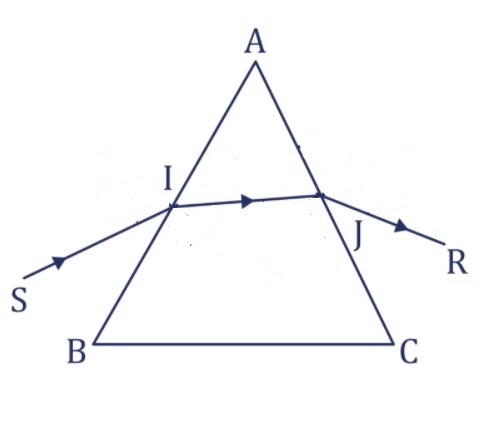
\includegraphics[scale=0.4]{../figs/VN12-PH-32-L-019-1-1.jpg}
\end{center}

Góc tạo bởi tia ló và tia tới gọi là \textit{góc lệch $D$} của ánh sáng khi truyền qua lăng kính.
\manatip{Khi không xảy ra phản xạ toàn phần, tia ló bao giờ cũng lệch về phía đáy lăng kính.}	
\subsubsection{Công thức của lăng kính}
\begin{center}
	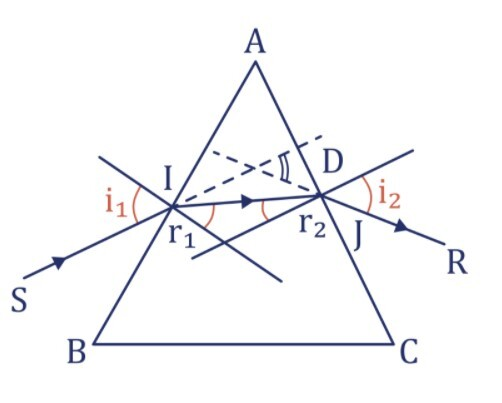
\includegraphics[scale=0.45]{../figs/VN12-PH-32-L-019-1-2.jpg}
\end{center}
\begin{itemize}
	\item Tại I: $\sin i_1=n\sin r_1$.
	\item Tại J: $\sin i_2=n\sin r_2$.
	\item Góc chiết quang: $A=r_1+r_2$.
	\item Góc lệch của tia sáng qua lăng kính: $D=i_1+i_2-A$.
\end{itemize}

\luuy{
	Nếu các góc nhỏ hơn $10^\circ$ thì công thức gần đúng của lăng kính là:
	\begin{itemize}
		\item $i_1=nr_1$,
		\item $i_2=nr_2$,
		\item $A=r_1=r_2$,
		\item $D=(n-1)A$.
	\end{itemize}
}

\subsection{Sự tán sắc ánh sáng}
\begin{center}
	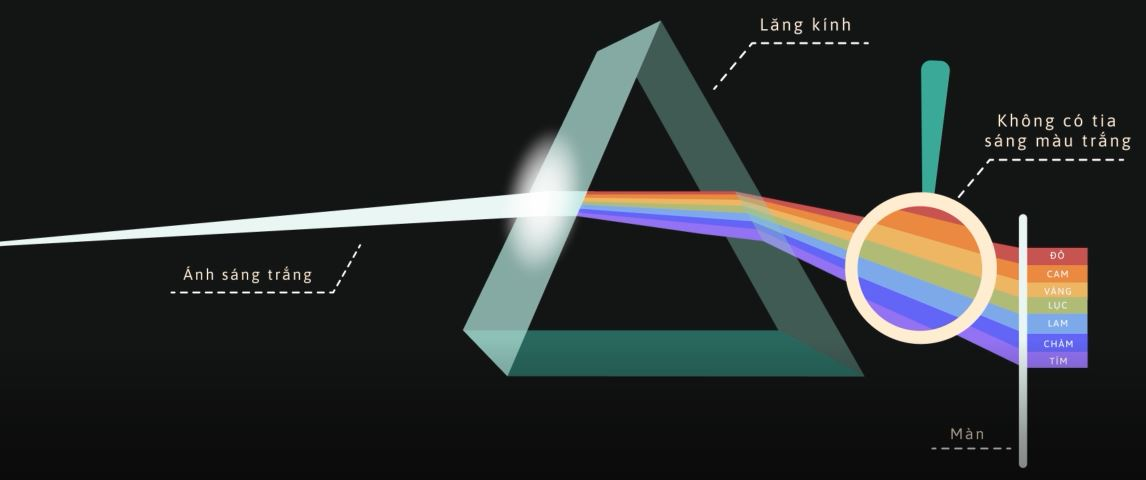
\includegraphics[width=\linewidth]{../figs/VN12-PH-32-L-019-1-3.jpg}
\end{center}

\begin{description}
	
	\item[Sự tán sắc ánh sáng] là sự phân tách một chùm sáng phức tạp thành các chùm sáng đơn sắc.
	\item[Ánh sáng đơn sắc] là ánh sáng có một màu nhất định và không bị tán sắc khi qua lăng kính.
	\item[Ánh sáng trắng] là hỗn hợp của nhiều ánh sáng đơn sắc có màu biến thiên liên tục từ màu đỏ đến màu tím. 
	\item[Chiết suất của thủy tinh] đối với các ánh sáng đơn sắc khác nhau thì khác nhau. Chiết suất có giá trị nhỏ nhất đối với ánh sáng đỏ và tăng dần khi chuyển sang màu da cam, màu vàng, ... và có giá trị lớn nhất đối với ánh sáng tím. Đặc điểm này là chung cho mọi chất trong suốt ($n_{\text{đ}}\leq n \leq  n_{\text{t}} $).
\end{description}
	
%		\luuy{ Mỗi ánh sáng đơn sắc có một tần số xác định}









	

